%!TEX root = ../march2025poster.tex

\begin{block}{Motivation and Background}
	
\textbf{Importance of Forecasting}
\begin{itemize}
	\item Influenza places a significant disease burden on temperate countries in the Northern Hemisphere every winter
	\item Accurate forecasts can help hospitals prepare for spikes and decide how to ration medication, and can impact how individuals make decisions regarding vaccination, mask wearing, travel, etc.
\end{itemize}
	
\textbf{Original motivating questions}
	\begin{itemize}
		\item How do scoring rules (explicit or implicit) potentially impact infectious disease forecasting competition submissions?
		\begin{itemize}
			\item[$\cdot$] Frongillo [3] studied how improper scoring rules can incentivize forecasters to report predictions that do not align with their true beliefs - could this be affecting the submissions to disease forecasting competitions?
		\end{itemize}
	\item CDC organizes the FluSight competition and uses the multibin logarithmic scoring rule, which is not proper [1]
		\item What is the optimal way to aggregate ensemble forecasts? 
		\begin{itemize}
			\item[$\cdot$] CDC currently seems to just take the median
		\end{itemize}
	\end{itemize}	

\textbf{Currect Project}
\begin{itemize}
	\item Goal: Forecast flu incidence at the state level using climate data
	\item Cold and dry conditions have been shown to correlate with increased flu (and other respiratory infection) activity [2]
	\item  Can incorporating climate data improve flu forecasts? 
\end{itemize}
\end{block}

\vspace{\colonesep}

\begin{block}{Methods}
\textbf{Step 1: Calculate ILI plus}
\begin{itemize}
	\item CDC collects data on percent of healthcare visits due to influenza-like illness (ILI) by state and publishes it weekly
	\item Report percent of flu tests that are positive by state each week
	\item As in Goldstein et al. [4], we use the product of percent visits due to ILI and percent positive flu tests as a proxy for flu incidence, which we call ILI plus
\end{itemize}

\textbf{Step 2: Fit a piecewise linear functions}
\begin{itemize}
	\item Since we expect flu incidence to grow and decay exponentially, we expect the log of ILI plus to grow and decay linearly
	\item For each flu season and state, fit a piecewise linear function with two breaks to the log of ILI plus data
	\item Record up slope, down slope, peak week, and peak value
\end{itemize}
\begin{center}
	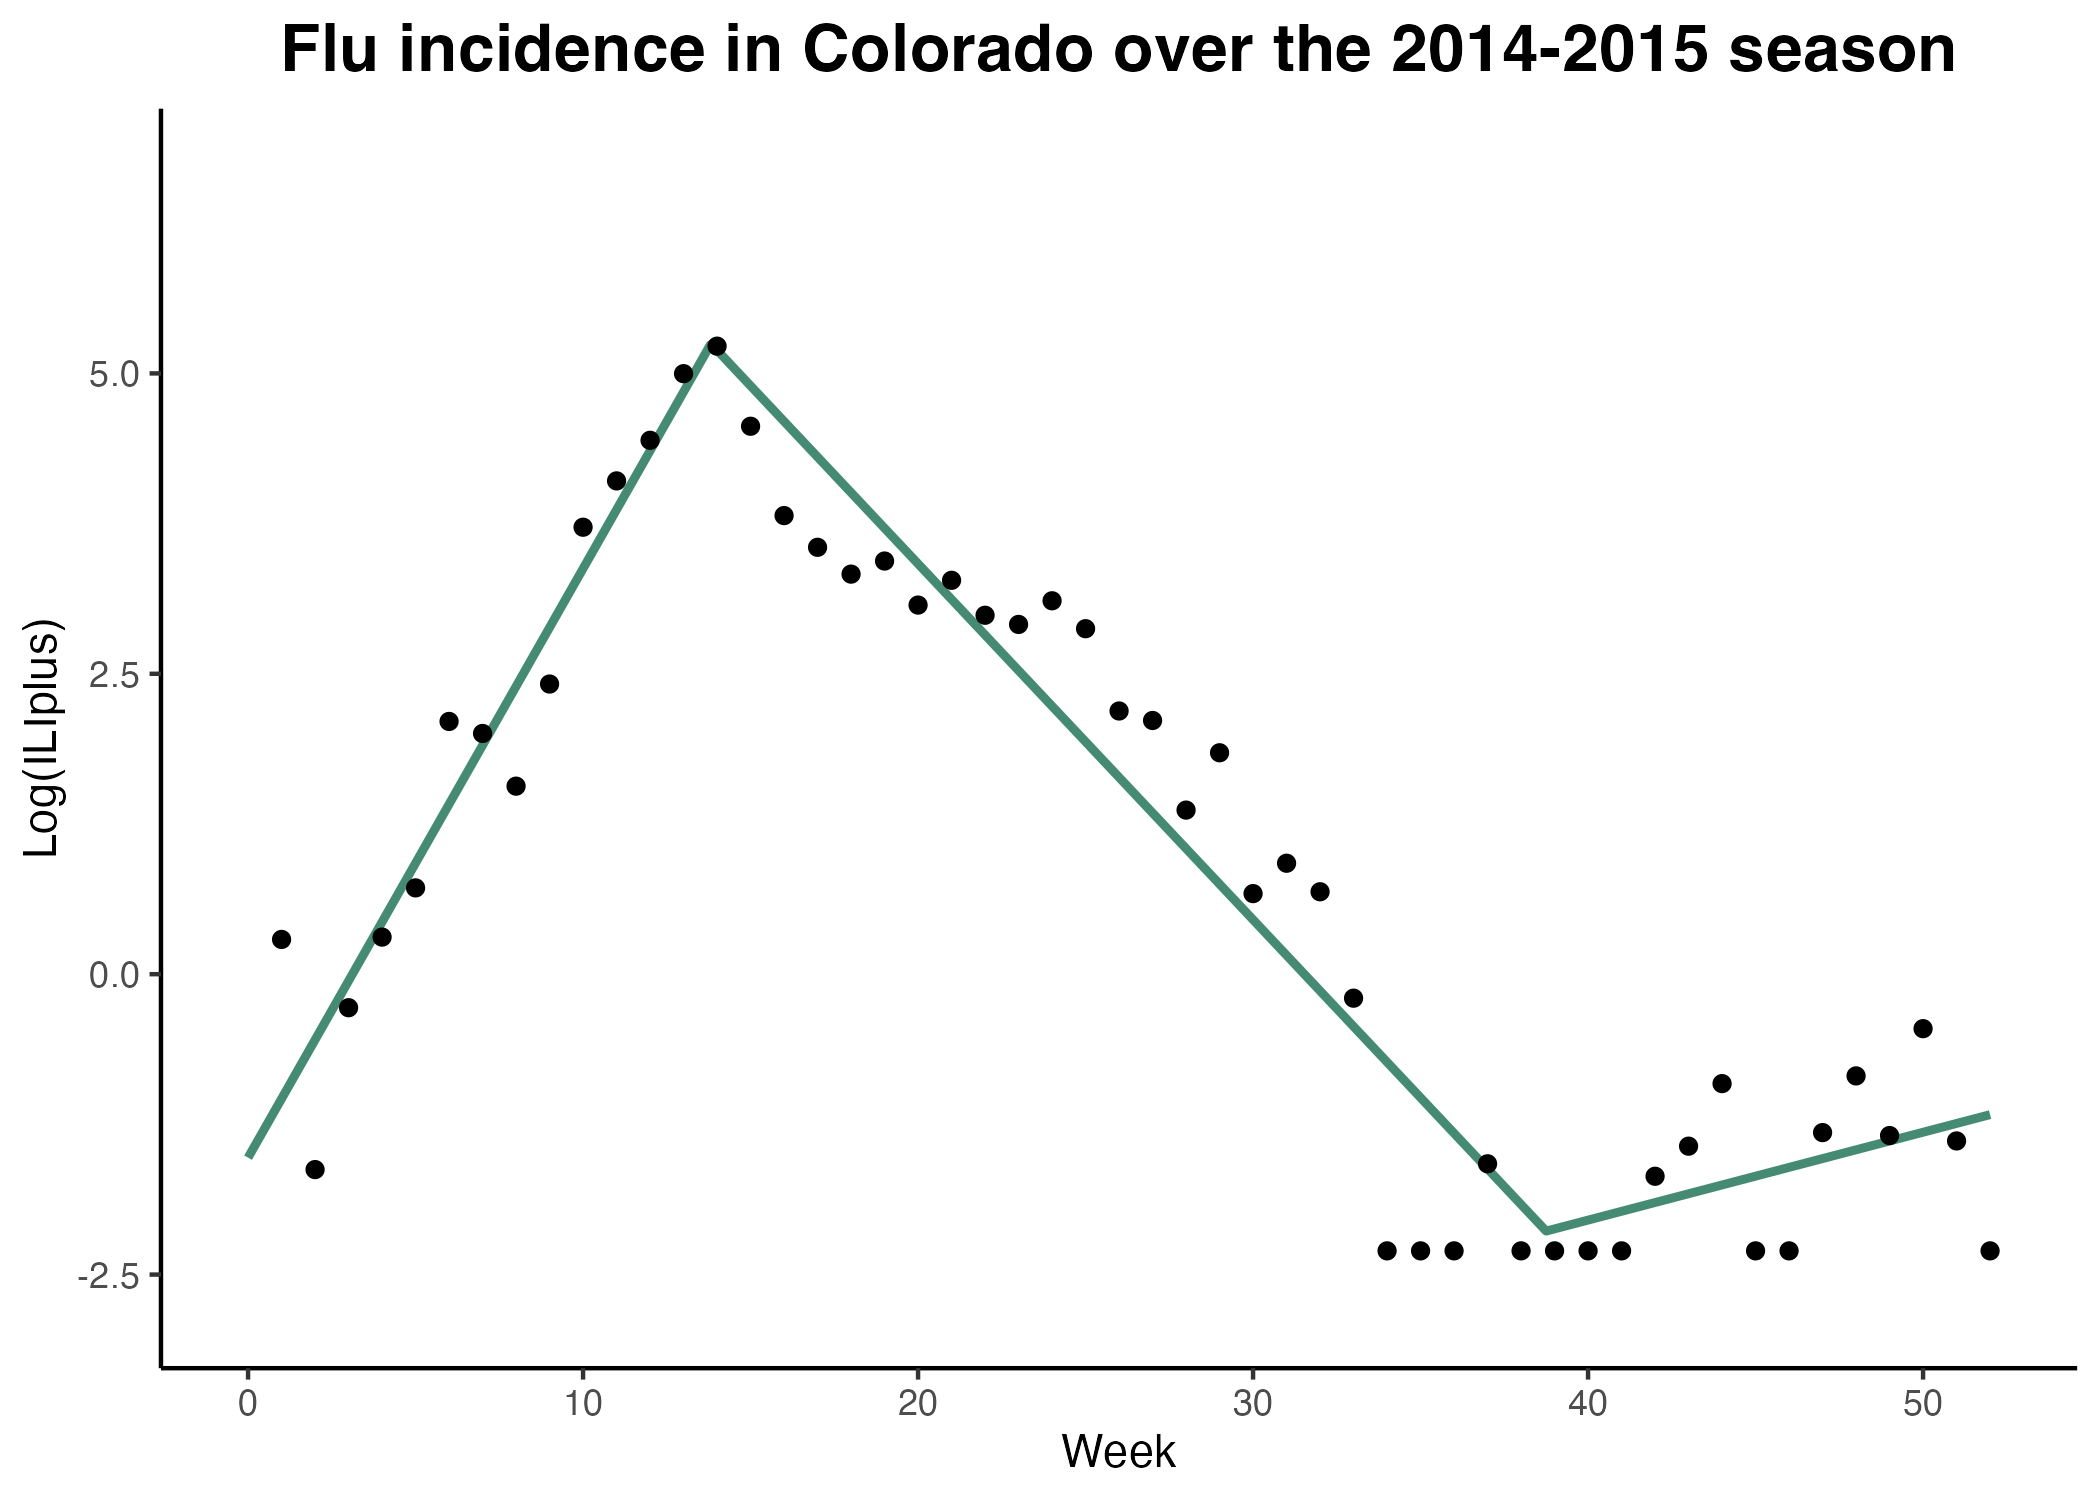
\includegraphics[width = 0.59\columnwidth]{sections/images/Colorado2014(just-fit).png}
\end{center}
\end{block}
